% !TEX root = index.tex

\section{Gluing it Back Together}
\epigraph{The only way to learn mathematics is to do mathematics.}{Paul Halmos}
\begin{align*}
 \xymatrix@R-2pc{
\U \ar@{~>}[r] & \L^\bullet(\U) \ar@{~>}[r] & \check H^*(X)\\
 \mbox{Good cover of } X & \mbox{Cech Complex of } \U & \mbox{Cech Cohomology of } X
 }
\end{align*}
We'll now associate to any cover $\U$ a cochain complex called the \textbf{Cech complex} $\L^{\bullet}(\U)$. To define the complex we need two things:
\begin{alignat*}{4}
	&\mbox{the spaces: } &&& \L^i(\U)\\
	&\mbox{the maps: } &&& d^i: \L^i(\U) \rightarrow \L^{i+1}(\U)
\end{alignat*}

\begin{definition}
	The \textbf{direct sum} $V \oplus V'$ of vector spaces $V$ and $V'$ with basis $\B$ and $\B'$ is a vector with basis the disjoint union $\B \sqcup \B'$.
\end{definition}
\noindent \textbf{Caution:} The disjoint union $\{1,2 \} \sqcup \{1,3\}$ equals $\{1, 2, 1', 3 \}$ and is different from the union $\{1, 2, 3 \}$. We keep both the copies of 1. Hence, ${\dim (V \oplus V') = \dim V  + \dim V'}$.

\begin{ques} $ $
	\begin{enumerate}
		\item What is $V \oplus 0$? Is $V \oplus V \cong V$?
		\item What is the relationship between $\dim V$, $\dim V'$ and $\dim (V \oplus V')$?
		\item Does the set of all vector spaces form a group under $\oplus$?
		\item Construct $\R^n$ using direct sums.
	\end{enumerate}
\end{ques}

\subsection{The Spaces}
Recall that to every subset $ I \subseteq [n]$ we can associate an open set $U_I $ defined as
\begin{align*}
	U_I := \bigcap_{i \in I} U_i
\end{align*}
For good covers, the connected components of $U_I$ are contractible.

\begin{definition}
	For $ 0 \le k < n$, let $(U_{I_1}, U_{I_2}, \dots, U_{I_m})$ denote the non-empty sets $U_I$ with $|I| = k+1$. Define
	\begin{align*}
		\L^k(\U) := \L(U_{I_1}) \oplus \L(U_{I_2}) \oplus \dots \oplus \L(U_{I_m})
	\end{align*}
\end{definition}
\begin{example}
  \label{ex:triangle_2}
	For the triangle with cover the three sides $U_1, U_2, U_3$
  \begin{align*}
		|I| = 0 &  & U_1, U_2, U_3                         \\
		|I| = 1 &  & U_{\{1,2\}}, U_{\{2,3\}}, U_{\{1,3\}}
	\end{align*}
	\begin{center}
		\begin{tabular}{l c l c l }
			$\L^0(\U)$ & : & $\L(U_1) \oplus \L(U_2) \oplus \L(U_3)$ & = & $\F^3$\\
			$\L^1(\U)$ & : & $\L(U_{\{1,2\}}) \oplus \L(U_{\{1,3\}}) \oplus \L(U_{\{2,3\}})$ & = & $\F^3$\\
			$\L^2(\U)$ & : & $\L(U_{\{1,2,3\}})$ & = & 0\\
		\end{tabular}
	\end{center}
	\begin{figure}[H]
		\centering
		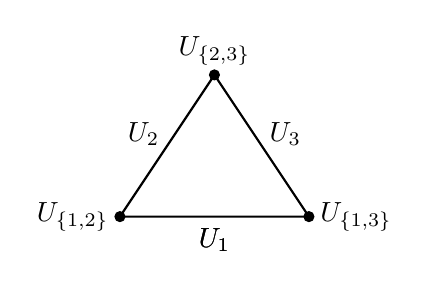
\begin{tikzpicture}[scale=0.6]
			%% vertices
			\draw[fill=black] (0,0) circle (3pt);
			\draw[fill=black] (4,0) circle (3pt);
			\draw[fill=black] (2,3) circle (3pt);
			%% vertex labels
			\node at (2,-0.5) {$U_1$};
			\node at (0.5,1.75) {$U_2$};
			\node at (3.5,1.75) {$U_3$};
			\node at (2,-0.5) {$U_1$};
			\node at (-1,0) {$U_{\{1,2\}}$};
			\node at (5,0) {$U_{\{1,3\}}$};
			\node at (2,3.5) {$U_{\{2,3\}}$};
			%%% edges
			\draw[thick] (0,0) -- (4,0) -- (2,3) -- (0,0);
		\end{tikzpicture}
		\caption{$\U = \{U_1, U_2, U_3\}$ is a good cover of the triangle, $U_{\{1,2\}}, U_{\{2,3\}}, U_{\{1,3\}}$ are the vertices, and $U_{\{1,2,3\}}$ is empty.}
		\label{fig:triangle_cech}
	\end{figure}
	So that the cochain complex (without the differentials) looks like
	\begin{align*}
		\L^\bullet(\U) = \xymatrix{ 0 \ar[r] & \F^3 \ar[r] & \F^3 \ar[r] & 0 }
	\end{align*}
\end{example}

\begin{ques}
	Find the Cech complex $\L^\bullet(\U)$ (without the differentials) for each of the following spaces using your favorite good cover $\U$. Compute the Euler characteristic $\chi$ of each of the spaces. (Note that you don't need to know the differentials $d^i$ to compute $\chi$.)
	\begin{multicols}{2}
		\begin{enumerate}
			\item $ \R^n$
			\item $ S^1$ (= the circle)
			\item A Tree
			\item The bipartite graph $ K_{2,3}$
			\item $ \R^2 \setminus \{(0,0) \}$
			\item $ \R^2 \setminus \{(0,0), (1,0), \dots, (k,0) \}$
			\item $S^1 \sqcup S^1$ (disjoint union of 2 circles)
			\item $S^1 \vee S^1$
			\item $ S^2 $ minus a point
			\item $ S^2 $ minus 2 points
		\end{enumerate}
	\end{multicols}
\end{ques}


\subsection{The Maps $d^i$}
The maps $d^i$ are simply the restriction maps $\res$ as defined in Question \ref{q:restrictions}.
\begin{ques}**
  Describe $d^i$ as a matrix in the canonical bases without looking at the next page (which has the answer). Find the differential $d^i$ in Example \ref{ex:triangle_2}.
\end{ques}
\newpage

\noindent In the canonical bases $d^i: \L^i(\U) \rightarrow \L^{i+1}(\U)$ is a matrix whose
\begin{enumerate}
  \item Rows correspond to the number of connected components of $U_I$ for all $|I|=i+2$
  \item Columns correspond to the number of connected components of $U_J$ for all $|J| = i+1$
  \item The $(i,j)^{th}$ entry is 1 if and only if the $i^{th}$ connected component of $U_I$ contains the $j^{th}$ connected component of $U_J$.
\end{enumerate}
\begin{example}
  \label{ex:triangle_cech}
	For a triangle in Figure \ref{fig:triangle_cech} we have inclusions $U_{\{1,2\}} \subseteq U_1$ etc., hence the differential $d^0$ looks like
	\begin{center}
		\begin{tabular}{ l | c c c  }
			& $U_1$ & $U_2$ & $U_3$ \\\hline
			$U_{\{1,2\}}$ & 1 & 1 & 0 \\
			$U_{\{2,3\}}$ & 0 & 1 & 1 \\
			$U_{\{1,3\}}$ & 1 & 0 & 1
		\end{tabular} $ = d^0$
	\end{center}
  So that
    \begin{align*}
  		\L^\bullet(\U)
      &=
      0 \rightarrow \F^3 \xrightarrow{\begin{bmatrix}1 & 1 & 0 \\0 & 1 & 1 \\ 1 & 0 & 1 \end{bmatrix}} \F^3 \rightarrow 0
  	\end{align*}
  \end{example}

  \begin{example}
    For the circle $S^1$ we can find a good cover consisting of two (slightly overlapping) semicircles.
    \label{ex:circle_cech}
    \begin{figure}[H]
  		\centering
  		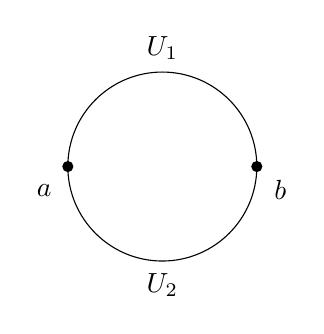
\begin{tikzpicture}[scale=0.6]
  			%% vertices
        \draw (2,2) circle (2cm);
  			\draw[fill=black] (0,2) circle (3pt);
        \draw[fill=black] (4,2) circle (3pt);
        \node at (2,4.5) {$U_1$};
        \node at (2,-0.5) {$U_2$};
        \node at (-0.5,1.5) {$a$};
        \node at (4.5,1.5) {$b$};
  		\end{tikzpicture}
  		\caption{$\{U_1, U_2\}$ is a good cover of the circle with $U_{\{1,2\}} = \{ a, b \}$}
  		\label{fig:triangle_cech}
  	\end{figure}
    \begin{align*}
  		|I| = 0 &  & U_1, U_2                         \\
  		|I| = 1 &  & U_{\{1,2\}}
  	\end{align*}
  	\begin{center}
  		\begin{tabular}{l c l c l }
  			$\L^0(\U)$ & : & $\L(U_1) \oplus \L(U_2)$ & = & $\F^2$\\
  			$\L^1(\U)$ & : & $\L(U_{\{1,2\}})$ & = & $\F^2$
  		\end{tabular}
  	\end{center}

    \end{example}


















\iffalse
\begin{example}
  \label{ex:triangle_cech}
	For a triangle in Figure \ref{fig:triangle_cech} we have the following non-empty sets
	\begin{align*}
		|I| = 0 &  & U_1, U_2, U_3                         \\
		|I| = 1 &  & U_{\{1,2\}}, U_{\{2,3\}}, U_{\{1,3\}}
	\end{align*}
	Hence the spaces in the chain complex are
	\begin{align*}
		0 \rightarrow \F^3 \rightarrow \F^3 \rightarrow 0
	\end{align*}
	Because of the non-empty inclusions $U_{\{1,2\}} \subseteq U_1$ etc. the differential looks like
	\begin{center}
		\begin{tabular}{ l | c c c  }
			& $U_1$ & $U_2$ & $U_3$ \\\hline
			$U_{\{1,2\}}$ & 1 & 1 & 0 \\
			$U_{\{2,3\}}$ & 0 & 1 & 1 \\
			$U_{\{1,3\}}$ & 1 & 0 & 1
		\end{tabular}
	\end{center}
  So that
    \begin{align*}
  		\L^\bullet(\U)
      &=
      0 \rightarrow \F^3 \xrightarrow{\begin{bmatrix}1 & 1 & 0 \\0 & 1 & 1 \\ 1 & 0 & 1 \end{bmatrix}} \F^3 \rightarrow 0
  	\end{align*}
  \end{example}

\begin{ques}
Compute the cohomology of the Cech Complex found in Example \ref{ex:triangle_cech}.
\end{ques}

\begin{ques}
  Find $\check H(-)$ for the following spaces.
  \begin{multicols}{2}
    \begin{enumerate}
      \item $ \R^m$
      \item $ S^1 = $ the circle
      \item A Tree
      % \item The bipartite graph $ K_{2,3}$
      \item $ \R^2 \setminus \{(0,0) \}$
      % \item $ \R^2 \setminus \{(0,0), (1,0), \dots, (k,0) \}$ for some positive integer $ k$
      \item $ S^2 $ minus a point
      \item $ S^2 $ minus 2 points
    \end{enumerate}
  \end{multicols}
\end{ques}

\begin{ques}
  Find the cohomology of a finite planar graph (thought of as a subset of $\R^2$).
\end{ques}
\fi
